\documentclass[30pt,twocolumn,letterpaper]{article}
\usepackage{cvpr}
\usepackage{times}
\usepackage{booktabs}
\usepackage{epsfig}
\usepackage{graphicx}
\usepackage{amsmath}
\usepackage{amssymb}
\cvprfinalcopy
\def\cvprPaperID{****}
\def\httilde{\mbox{\tt\raisebox{-.5ex}{\symbol{126}}}}
\usepackage{graphicx}
\usepackage{indentfirst}
\setlength{\parindent}{2em}
\usepackage{cite}
\usepackage[colorlinks,linkcolor=red,anchorcolor=blue,citecolor=green,backref=page]{hyperref}
\author{Qilei Zhang\\\\
Jul 10 2018}
\title{What do 15,000 object categories tell us about classifying and localizing actions?}
\begin{document}
\maketitle
\begin{abstract}
  This paper helps to automatically classify and localize human behavior in video. Motion is the key component of modern methods. Evaluation has the advantages of objects in video representation. Instead of taking into account a few carefully selected and localized objects, the benefits encoding the positive study of the 15000 object categories use 6 data sets, totaling more than 200 hours of video and covering 180 action classes.
\end{abstract}
\section{Introduction}
It helps to automatically classify and locate human behaviors, such as telephone, horse riding and sumo wrestling video content. Unlike the leading technologies in these two challenging problems, research has the benefits of objects in video representation. For action classification, the relationship between objects and actions has been considered earlier, but only for a few selected and localized objects\cite{Hazelhoff2015Large}. \\
\begin{figure}[htbp]
\small
\centering
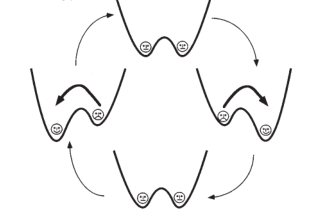
\includegraphics[width=20em]{000.png}
\caption{In this paper we ask ourselves the question: ��What do
15,000 object categories tell us about classifying and localizing
actions?�� and conduct an empirical study on the benefit of encoding
object categories for action. We show that: objects matter for
actions, actions have object preference, object-action relations are
generic, and adding object encodings improves the state-of-the-art
in action classification and localization.
}
\label{fig:lable}
\end{figure}\\
\section{Related work}
Advancements in action classification have resulted in a mature repertoire of elegant and reliable techniques yielding good accuracy. Such techniques include sampling at interest points, densely or along dense trajectories. Such samples are represented by powerful local descriptors which are robust to modest appearance and motion changes\cite{Huang2015Fin}.\\
\begin{figure}[htbp]
\small
\centering
\includegraphics[width=20em]{001.png}
\caption{Action examples from the UCF101, THUMOS14, Hollywood2, HMDB51, UCF Sports and KTH
datasets that we consider in our empirical study to reveal what 15,000 object categories tell us about classifying and localizing actions.
}
\label{fig:lable}
\end{figure}\\
\section{Conclusion}
Experiments show that objects matter for actions, and are often semantically relevant as well, especially when the actions interact with objects. What is more, the object representation is complementary to modern motion encodings\cite{Jagadeesh2014Synapse}.\\
\par
The determination of action has an object preference. Instead of using all objects, selection is advantageous in terms of compact video representation, as well as in its discriminative action classification ability. The object action relation of learning is universal and transferred from one data set to another. When object representation is combined with modern motion coding and space-time action proposals, it leads to the action classification and localization of the most advanced five data sets in a new country.
{\small
\bibliographystyle{ieee}
\bibliography{1}
}
\end{document}
